
% *************************************************************************
% You can now use this template both for submitting to peer review and,
% if your paper is accepted, for sending in final publication materials.
% To change from peer review format (single column, double-spaced) to
% final publication format (double column, single-spaced), just move the
% comment-line sign (%) from one \documentclass line to the other.
% The first is for peer review format(single column), the second is for final publication(double column).
\documentclass[12pt,journal,draftcls,letterpaper,onecolumn]{IEEEtran}
%\documentclass[9.5pt,journal,final,finalsubmission,twocolumn]{IEEEtran}
%\documentclass[9.5pt,journal,letterpaper,compsoc,peerreview]{IEEEtran}
\usepackage{pifont}
\usepackage{multirow}
\usepackage{comment}
\usepackage{subfigure}
\usepackage{color}
\usepackage{epsfig}
\usepackage{times}
\usepackage{url}
\usepackage{lineno}
\usepackage[nocompress]{cite}
% *************************************************************************


\usepackage{amsmath}   % From the American Mathematical Society
                        % A popular package that provides many helpful commands
                        % for dealing with mathematics. Note that the AMSmath
                        % package sets \interdisplaylinepenalty to 10000 thus
                        % preventing page breaks from occurring within multiline
                        % equations. Use:
%\interdisplaylinepenalty=2500
                        % after loading amsmath to restore such page breaks
                        % as IEEEtran.cls normally does. amsmath.sty is already
                        % installed on most LaTeX systems. The latest version
                        % and documentation can be obtained at:
                        % http://www.ctan.org/tex-archive/macros/latex/required/amslatex/math/


\begin{document}
%
% paper title
\title{A novel heuristic for local multiple alignment of interspersed DNA repeats}
%
%
% author names and IEEE memberships
% note positions of commas and nonbreaking spaces ( ~ ) LaTeX will not break
% a structure at a ~ so this keeps an author's name from being broken across
% two lines.
% use \thanks{} to gain access to the first footnote area
% a separate \thanks must be used for each paragraph as LaTeX2e's \thanks
% was not built to handle multiple paragraphs
\author{\ \ }

% The paper headers
%\markboth{Journal of \LaTeX\ Class Files,~Vol.~1, No.~8,~August~2002}{Shell \MakeLowercase{\textit{et al.}}: Bare Demo of IEEEtran.cls for Journals}
% The only time the second header will appear is for the odd numbered pages
% after the title page when using the twoside option.

% use only for invited papers
\IEEEspecialpapernotice{(Invited Paper)}

% make the title area
\maketitle
\linenumbers 
%\IEEEdisplaynotcompsoctitleabstractindextext
%\IEEEcompsoctitleabstractindextext{
\begin{abstract}
Pairwise local sequence alignment methods have been the prevailing technique to identify homologous nucleotides between related species. However, existing methods that identify and align all homologous nucleotides in one or more genomes have suffered from poor scalability and limited accuracy. We propose a novel method that couples a gapped extension heuristic with an efficient filtration method for local multiple alignment.  During gapped extension, we use the MUSCLE implementation of progressive multiple alignment with iterative refinement.  The resulting gapped extensions potentially contain alignments of unrelated sequence.  We detect and remove such undesirable alignments using a hidden Markov model to predict the posterior probability of homology. The HMM
emission frequencies for nucleotide substitutions can be derived from any strand/species-symmetric nucleotide substitution matrix, and we have developed a method to adapt an arbitrary substitution matrix
to organisms with different G+C content. We evaluate the performance of our method and previous approaches on a hybrid dataset of real genomic DNA with simulated interspersed repeats.  Our method
outperforms a related method in terms of sensitivity, positive predictive value, and localizing boundaries of homology. In addition, we present a statistical test for estimating significance of local multiple alignments. The described methods have been implemented in freely available software,\texttt{Repeatoire}, available from: \url{http://wwwabi.snv.jussieu.fr/public/Repeatoire}
\end{abstract}

\begin{IEEEkeywords}
Sequence alignment, genome comparison, DNA repeats, local multiple alignment, hidden Markov model, gapped extension
\end{IEEEkeywords}

\IEEEpeerreviewmaketitle
\section{Introduction}
Pairwise local sequence alignment has a long and fruitful history in computational biology and new approaches continue to be proposed~\cite{ref-pattern,ref-chaos,ref-yass,ref-kahveciMAP}. Advanced filtration methods based on spaced-seeds have greatly improved the sensitivity, specificity, and efficiency of many local alignment methods~\cite{ref-zhang04,ref-zhang06,ref-buhler05,ref-xu04,ref-batzoglouNAR, ref-rasmussen}. Common applications of local alignment range from orthology mapping~\cite{ref-orthomcl} to genome assembly~\cite{ref-arachne2} to information engineering tasks such as data compression~\cite{ref-ane}. Recent advances in sequence data acquisition technology~\cite{ref-454, sequencing, hybrid} (see ~\cite{ref-nextgenseq} for a recent review) provide low-cost sequencing and will continue to fuel the growth of molecular sequence databases. To cope with advances in data volume, corresponding advances in computational methods are necessary; thus we present an efficient method for local multiple alignment of DNA sequence.

Unlike pairwise alignment, local multiple alignment constructs a single multiple alignment for all occurrences of a motif in one or more sequences.  The motif occurrences may be identical or have degeneracy in the form of mismatches and indels.  As such, local multiple alignments identify the basic repeating units in one or
more sequences and can serve as a basis for downstream analysis tasks such as multiple genome alignment~\cite{ref-mauve,ref-mga,ref-mgcat,ref-deweyReview}, global alignment with repeats~\cite{ref-otherSammethPaper,ref-aba}, or repeat classification and analysis~\cite{ref-piler}.  Local multiple alignment differs from traditional pairwise methods for repeat analysis which either identify repeat families \textit{de novo}~\cite{ref-reputer} or using a database of known repeat motifs~\cite{ref-repbase}.

The importance of accurate homology identification to comparative genomics can not be overestimated~\cite{Kumar07}. To date, pairwise local sequence alignment methods such as BLAST~\cite{ref-blastz,ref-ssearch} have been the prevailing technique to identify homologous nucleotides. When more than two copies of a homologous sequence element are present in the data, pairwise homology detection methods generate a listing of all possible pairs of homologous elements in the form of pairwise local alignments.  Apart from the obvious inefficiency of considering all pairwise homology relationships, a collection of pairwise alignments is not ideal because they are rarely amenable to comparative genomic and phylogenetic analysis without further processing into a multiple alignment.

Local pairwise alignments can be merged to create a multiple alignment by a variety of
methods~\cite{ref-tba,ref-dialign,ref-related1}. Such methods commonly assume that pairwise homology relationships are transitive, such that if nucleotide $a$ is homologous to nucleotide $b$, and $b$ is to $c$, then $a$ must also be homologous to $c$.  Thus, in order to merge pairwise alignments, such methods must tackle the challenging problem of resolving inconsistent transitive homology relationships.
Multiple alignment has been demonstrated to be more accurate than pairwise alignment, especially when dealing with a large number of divergent sequences~\cite{ref-mlagan,ref-aubergene}.  As the number of homologous sequences grows, we might expect that the number of inconsistent relationships in a collection of pairwise alignments would grow quadratically, whereas a direct multiple alignment method would provide an increasingly accurate alignment.  Moreover, highly repetitive regions in the input sequences can cause serious efficiency
problems for pairwise methods, as they create $O(r^{2})$ pairwise alignments in the presence of a repeat with $r$ copies.  Mammalian Alu repeats and IS (insertion sequence element) repeats in microbes are two common examples of the overwhelming abundance of repetitive sequence in whole genomes.

Local multiple alignment has the inherent potential to avoid pitfalls associated with pairwise alignment. Although optimal multiple alignment under the Sum-of-pairs objective function remains intractable~\cite{ref-wangjiang}, progressive alignment heuristics offer excellent speed and accuracy~\cite{ref-clustalw,ref-tcoffee} especially when combined with tree-independent iterative
refinement~\cite{ref-muscle}, or probabilistic consistency measures~\cite{ref-probcons}. In the context of \textit{local}
multiple alignment, the fundamental problem with such an approach is
that current methods for progressive alignment with iterative
refinement compute \textit{global} alignments, i.e. they implicitly
assume that input sequences are homologous over their entire length. 

\section{A heuristic for gapped extension of local multiple alignments}
We present a novel heuristic for directly computing local multiple alignments via gapped extension of chained seed matches. Our method for computing local multiple alignments utilizes the MUSCLE
multiple alignment algorithm to compute gapped extensions of ungapped
multi-match seeds (see Figure~\ref{fig-main}). Gapped alignments arise
when extending seed matches to fully capture surrounding sequence
homology. Our method first computes a
global multiple alignment on a dynamically calculated window of nucleotides
flanking a seed match.  However, as we do not know the boundaries of the
homologous sequence a priori, this approach may result in the
alignment of unrelated sequences.  To resolve the problem, we employ a hidden Markov model configured to detect
unrelated regions embedded in the global multiple alignment.
Unrelated regions are then removed from the alignment and the
local-multiple alignment is trimmed to reflect the updated boundaries
of homology.

Our method, depicted for an example sequence in
Figure~\ref{fig-main}, has six primary steps: (A) Identify
multi-match seeds in the input sequence, (B) Chain individual
seeds, (C) Perform multiple alignments on regions between chained seeds, (D)
Perform gapped extension of seed chains (E) Detect unrelated regions
using a hidden Markov model, and finally, (F) Trim any unrelated regions from
the final local multiple alignment. For steps (A) and (B), we employ the palindromic seed identification
and chaining algorithm implemented in our previous work (\texttt{procrastAligner}~\cite{ref-procrast}). The remaining steps are applied
repeatedly to seeds identified in step (A) to produce local multiple
alignments of all homologous nucleotides in the input sequence.


\subsection{Identifying multi-match seeds in the input sequence}
Given a sequence $\mathcal{S}=s_1, s_2,\dots, s_N$ of length $N$
defined over an alphabet $\{A,C,G,T\}$, our method first extracts candidate ungapped
alignments, or multi-matches, among subsequences in $\mathcal{S}$,
and we denote the set of all such matches as $\mathbf{M}$. To extract multi-matches from the input
sequence, we utilize a palindromic spaced seed pattern~\cite{ref-zhang}, which is
analyzed at each position in the input sequence.
Palindromic spaced seeds were presented our previous work and were shown to offer good efficiency and
reasonable sensitivity on a variety of input
sequences~\cite{ref-procrast}.  We refer the number of matching regions
in $\mathcal{S}$ by a given match $M_i \in \mathbf{M}$ as the
\textit{multiplicity} of $M_i$, denoted as $|M_i|$. We refer to each
matching region of $M_i$ as a \textit{component} of $M_i$. Our
algorithm has an important limitation on the matches in $\mathbf{M}$:
no two matches $M_i$ and $M_j$ may have the same left-end coordinate,
except for the identity case when $i=j$.  This constraint has been
referred to by others as \textit{consistency} and
\textit{transitivity}~\cite{ref-transitivity} of matches. Nevertheless,
after gapped extension, it is possible that two or more
local multiple alignments share the same left-end coordinate.



\begin{figure}[t!]
\begin{center}
%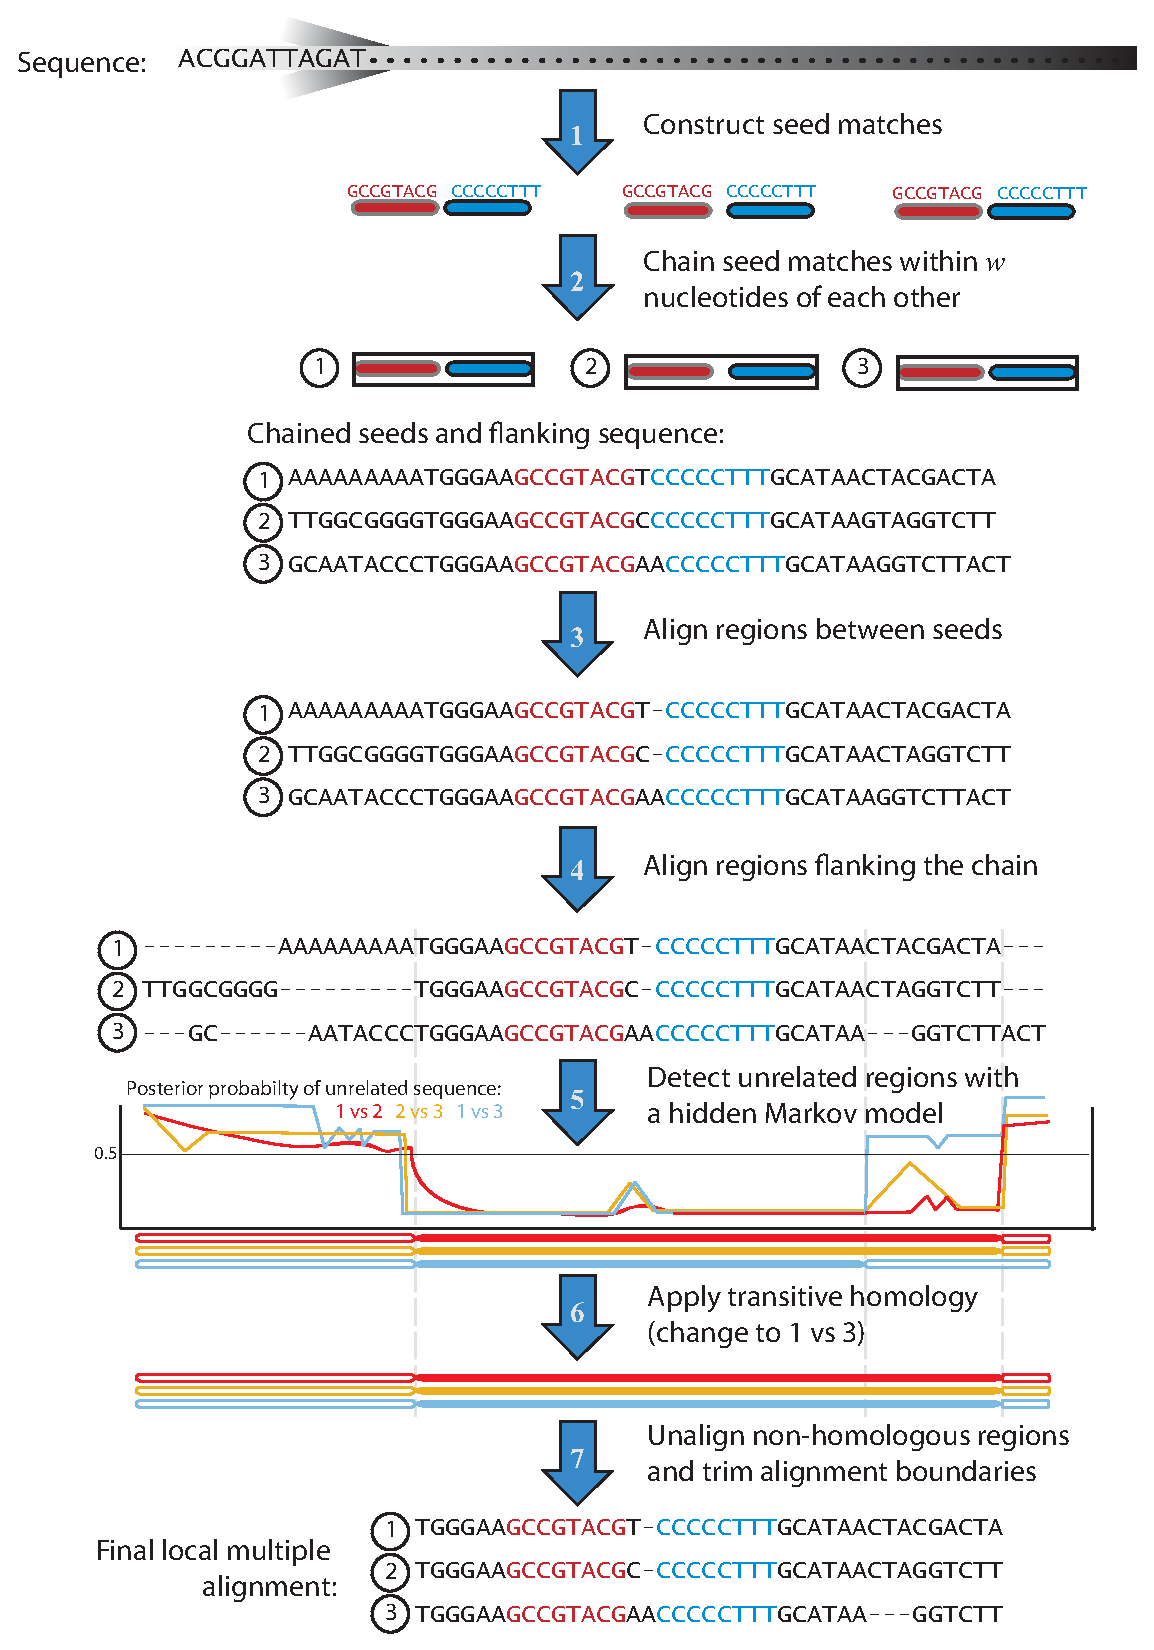
\epsfig{file=./fig/extension.eps,width=3.5in}
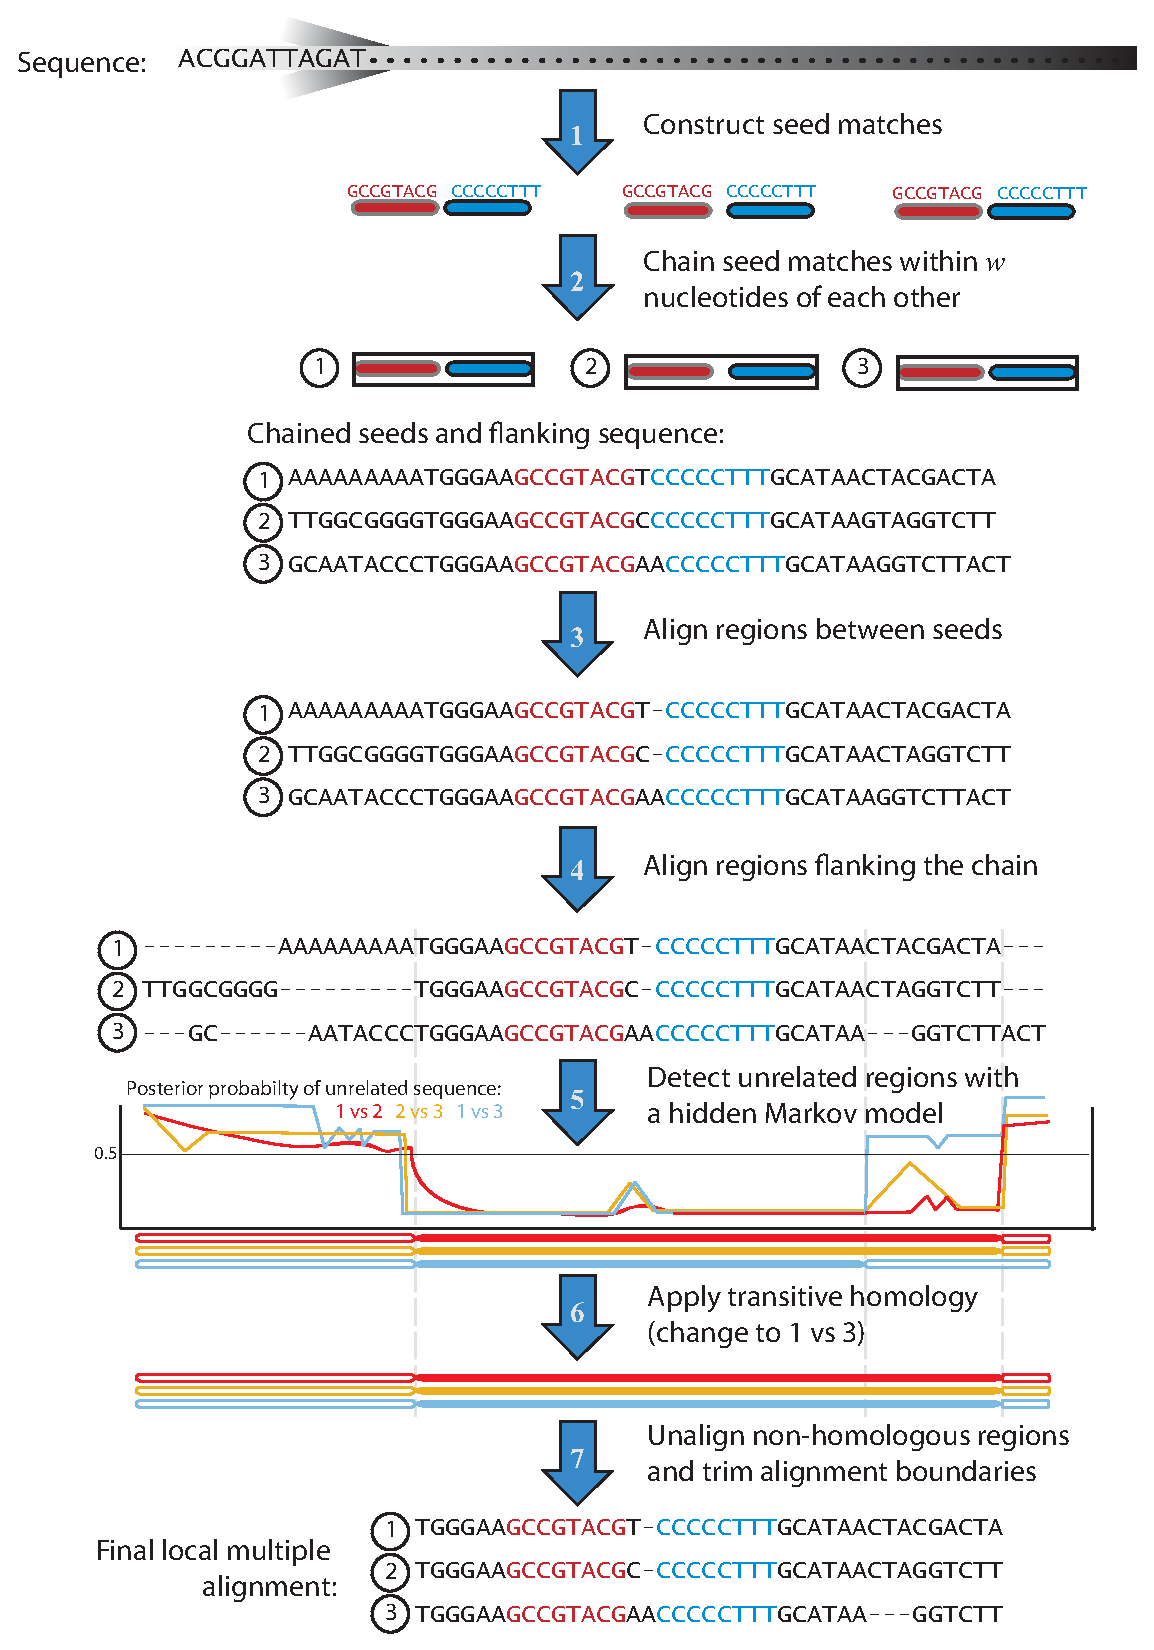
\epsfig{file=./fig/extension.eps,width=4.0in}
%\subfigure[Visual representation of our algorithm]{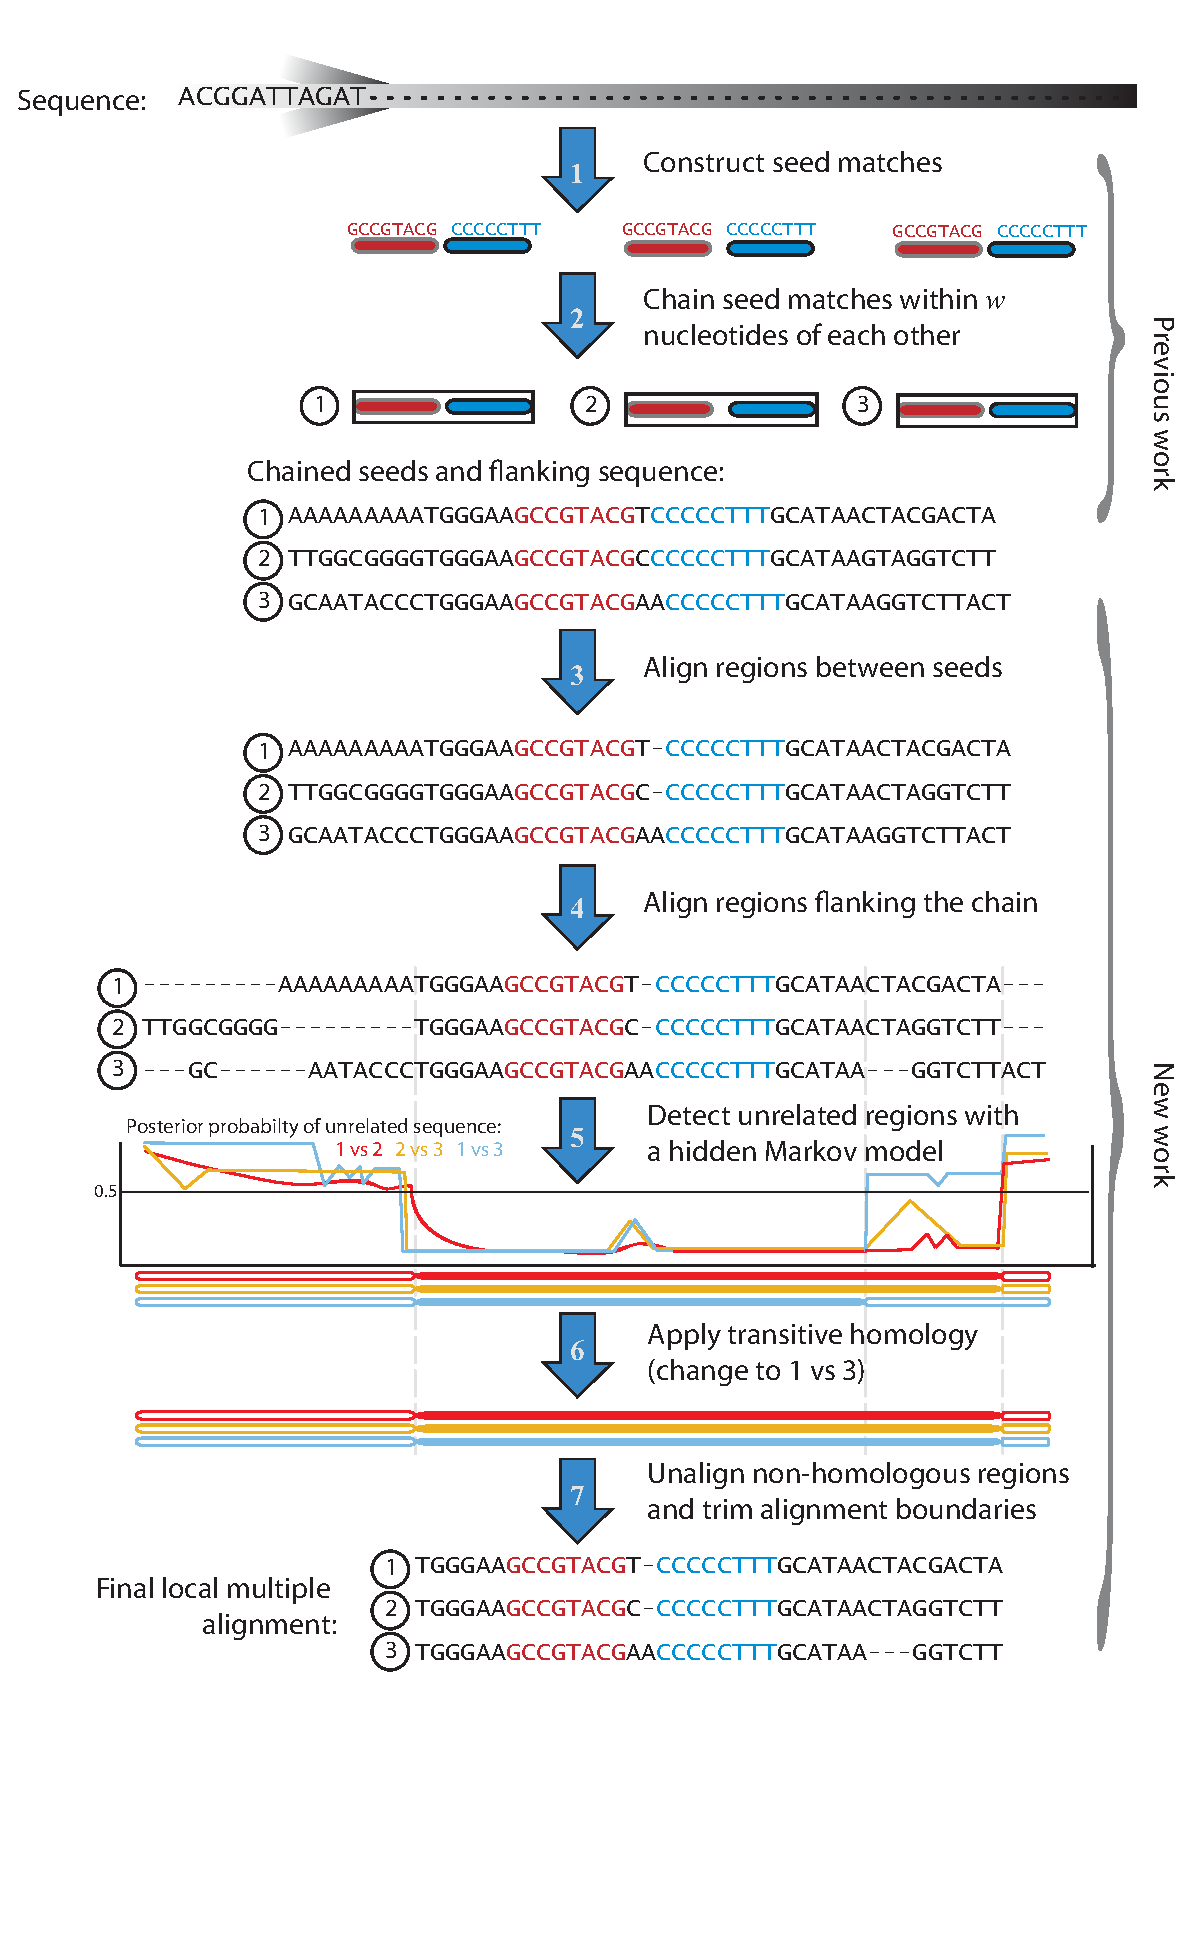
\epsfig{file=./figures/extension.eps,width=3.0in}}
%\subfigure[Flowchart of the algorithmic process ]{ 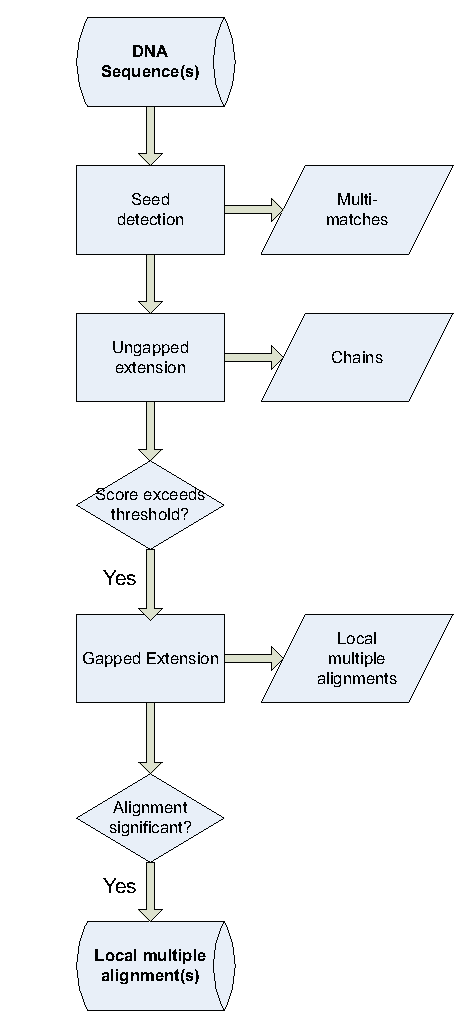
\epsfig{file=./figures/flowchart.eps,width=1.7in}}
\end{center}
%\vspace{-1.6cm}
\caption
{Overview of the method, starting with an input sequence and ending
with a set of local multiple alignments. First we (A) detect
multi-matches in the input sequence(s) using palindromic spaced seeds,
then we perform (B) chaining and extension of all multi-matches within
the distance of $w$ nucleotides of each other.  In the present example, one chain exists and
contains two matches each with three match components labeled 1, 2,
and 3.  We then perform gapped alignment of the region between chained
matches (C).  In step (D), we perform a gapped extension by computing
a global multiple alignment on the regions to the left and right of
each chain component.  The resulting alignment may contain unrelated
sequence, so in step (E) we apply a hidden Markov model to detect
poorly aligned regions indicative of unrelated sequence and
compute transitive homology relationships to ensure a consistent
alignment and aid detection of divergent homologous sequences.
Finally, in step (F) we unalign regions found to be non-homologous.
If we find after step (B) that the alignment boundaries have been
extended, we return to step (D) for another round of chaining.}
\label{fig-main}
\end{figure}

\subsection{Chaining multi-match seeds from the input sequence}
Once a list of multi-matches has been generated, we utilize an
efficient chaining and filtration algorithm to identify overlapping
and nested chains of multi-matches~\cite{ref-procrast}. In order to
process each region of sequence $\mathcal{O}(1)$ times, matches
are prioritized for chaining in order of decreasing $|M_i|$.  The
method chains multi-match seeds of the same $|M_i|$
occurring within $w$ characters of each other, thus gaps of up to size
$w$ are tolerated.  When a multi-match can
no longer be chained without including a gap larger than $w$
characters, neighboring \textit{subset} matches within $w$ characters
are identified. Each neighboring subset match is then \textit{linked}
to the chained match. We refer to the chained match as a
\textit{superset} match. Rather than immediately extend the subset
match(es), we \textit{procrastinate} and extend the subset match later
when it has the highest multiplicity of any match waiting to be
extended. When chaining a match with a linked superset, we immediately
include the entire region covered by the linked superset match and
thus eliminate the need to re-examine sequence already covered by a
previously chained match.

\subsection{Aligning regions between multi-match seed chains}
After chaining a multi-match $M_i$, we perform gapped global alignment via MUSCLE on all
collinear regions located between two adjacent multi-match components to generate
unextended local multiple alignments. As previously mentioned, the maximum length of the region to align
is controlled via the $w$ parameter. We have empirically determined that reasonable values
for $w$ in a wide variety of settings can range from 2 to 3 times the seed length. However, since this
parameter can be configured manually and large values of
$w$ could potentially result in aligning unrelated sequence, the HMM test (discussed in detail later) can be optionally applied
aligned regions between multi-match seeds to avoid aligning unrelated sequence. If the test detects any part of the 
region to be unrelated, the multi-match chain is broken and separated into two individual multi-matches.

\subsection{Gapped extension of high-scoring chains}
Next, our method computes gapped extensions of the chained multi-match seeds.
We can optionally require that two or more seeds be present
in the chain and use lower seed weights ($k$), a technique which has
previously been proven
successful~\cite{ref-blastz,ref-gappedblast,ref-blat}.  To perform a
gapped extension in each direction, we use MUSCLE to align dynamically-calculated window
of nucleotides ($l$) to the left and right of the current local
multiple alignment.  Small values of $l$ restrict the alignment search
space, while larger values require more computation but are
potentially more sensitive.  We have empirically determined that
setting $l$ based on multiplicity ($l = 70e^{-0.01*|M_{i}|}$) offers a
good tradeoff between speed and sensitivity.  The resulting extension
window is small for high multiplicity chains,
keeping the alignment search space tractable.
%\begin{equation}
% \max(w, \sqrt{(\max(150^{2}-(2*|M_{i}|)^{2},0)}));
%\end{equation}

\subsection{Detecting unrelated regions in the alignment}
\begin{figure*}[t!]
\centering 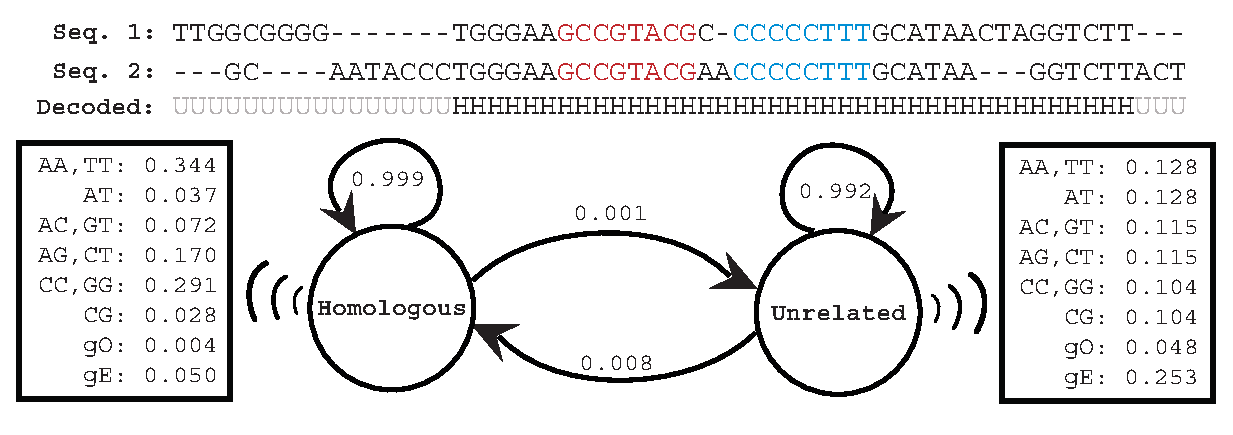
\epsfig{file=./fig/hmm.eps,width=6.8in}
\caption[Hidden Markov model used to detect pairwise alignments of unrelated
sequence]%
{\textbf{Hidden Markov model used to detect pairwise alignments of unrelated
sequence.} The HMM has states which model alignment columns containing
homologous and unrelated sequence. Emission probabilities are extracted from the HOXD70 substitution matrix and correspond to alignment
columns, for example \texttt{AA} indicates A aligned to A.  gO
indicates gap-open and gE gap extend. Alignment columns are treated as
strand-symmetric, so that AC also indicates CA and the reverse
complements TG and GT.  The emission probabilities are adjusted to the G+C content of the input genome
as described in the text.  The values shown here correspond to a 47.5\% G+C genome.}
\label{fig-hmm}
\end{figure*}
The MUSCLE alignment software reports the highest scoring
global multiple alignment of input sequences, regardless of whether
they are related by common ancestry. As a consequence of the gapped
extension process, it is possible that our method forcibly aligns unrelated
sequence. We have configured a hidden Markov model (Figure
~\ref{fig-hmm}) to detect alignments of unrelated sequence. The HMM
consists of two hidden states, Homologous and Unrelated. The
observable states are the pairwise alignment columns, which are all
possible pairs in $\texttt{{\{A,G,C,T,-\}}}$ with strand
symmetry and undirected changes, i.e. \texttt{AG=GA=TC=CT}. The emission probabilities for
each possible pair of aligned nucleotides were extracted from the HOXD70
substitution matrix presented by Chiaromonte \textit{et al.}~\cite{hoxd} :
\large
\begin{center}
\begin{equation}
\begin{array}{crrrr}
  & \texttt{A} & \texttt{C} & \texttt{G} & \texttt{T} \\
\texttt{A} & 91 & -114 & -31 & -123 \\
\texttt{C} & -114 & 100 & -125 & -31 \\
\texttt{G} & -31 & -125 & -100 & -114 \\
\texttt{T} & -123 & -31 & -114 & 91 \\ \end{array}
\end{equation}
\end{center}

\normalsize
We extracted the emission probabilities by solving for the emission frequencies in the
Homologous and Unrelated state using the same equation used to
calculate the values of the HOXD70 substitution matrix on 47.5\%G+C
content sequence~\cite{hoxd}:
\begin{equation}
s(x,y)= \log_{2}{\Bigg(\frac{p(x,y)}{q_{1}(x)q_{2}(y)}\Bigg)}
\end{equation}
{w}here $p(x,y)$ is the fraction of the observed aligned pairs of
nucleotides $x$ and $y$ in the training set used and $q_{1}(x)$ and
$q_{2}(x)$ denote the background frequencies of $x$ and $y$,
respectively. Chiaromonte \textit{et al.} scaled the resulting
$s(x,y)$ values so the largest was 100,
with the rest rounded to the nearest integer. The resulting emission
probabilities for the Homologous and Unrelated states are given
in Figure~\ref{fig-hmm} (see supplemental material for
more details on the derivation of the emission probabilities). 

The HMM probabilities can be derived using any nucleotide substitution matrix with  strand symmetry and undirected changes,
but any particular matrix makes specific assumptions about divergence time, mutation pressures,
and sequence composition of the aligned sequences.
Genomes can range in G+C content from 30-75\%, and at the extremes,
a substitution matrix derived on 47.5\% G+C sequence (such as HOXD70) does not
perform well. Previously it has been shown that adapting substitution matrices to the composition
of the organisms under comparison can improve sequence alignment accuracy~\cite{ref-rev3b}.  We have thus developed a method to adapt HMM emission
probabilities derived from an arbitrary substitution matrix
to organisms with different G+C content (see supplemental material).

While emission frequencies for nucleotide substitutions can be derived from
any any nucleotide substitution matrix with  strand symmetry and undirected changes, the gap-open
and extend frequencies can not.  To empirically estimate gap-open and extend values
for the unrelated state we aligned a 10-kb, 48\%~G+C content region
taken from \emph{E. coli} CFT073 (Accession AF447814.1, coordinates
37,300-38,300) with an unrelated sequence.  We generated an unrelated
sequence with identical nucleotide composition by randomly shuffling the
extracted sequence.  We then forced an
alignment with MUSCLE and counted the number of gap-open and gap-extend
columns in the alignment of unrelated sequences.  Gap-open and
extend frequencies for the homologous state were estimated by
constructing an alignment of 10kb of orthologous sequence shared among
a pair of divergent organisms.  We aligned the 48\%G+C segment between
genes \textit{fruR} and \textit{secA} from \textit{E. coli} K12
(Accession U00096.21) and \emph{Y. pestis} CO92 (Accession
AL590842.1). We add the empirically derived gap-open and extend
frequencies for each state and normalize the emission frequencies to a
probability distribution.  The resulting emission probabilities are
reported in Figure~\ref{fig-hmm}.


\begin{figure*}[t!]
\centering 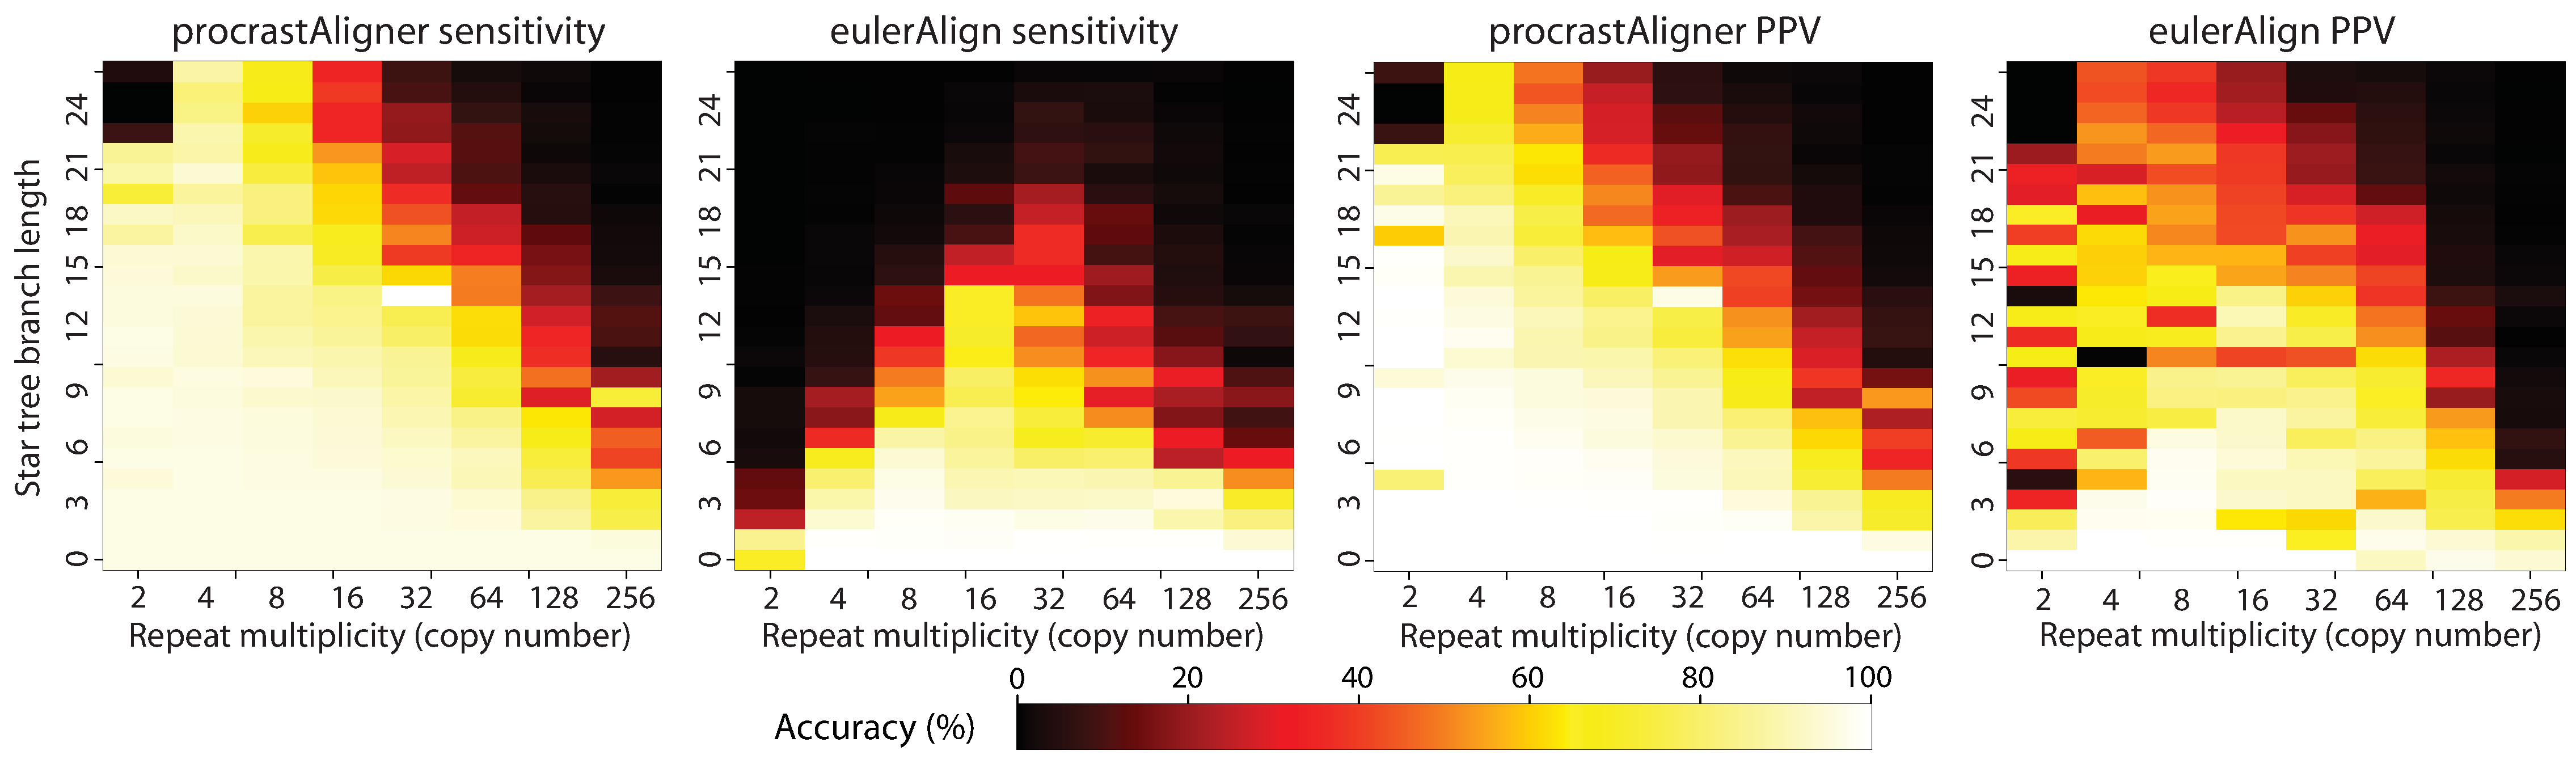
\epsfig{file=./fig/repeat_accuracy_new.eps,width=6.8in}
\caption[Accuracy recovering simulated repeat families planted in the
\textit{Mycoplasma genitalium} genome]%
{\textbf{Accuracy recovering simulated repeat families planted in the
\textit{Mycoplasma genitalium} genome}.  Sum-of-pairs nucleotide
sensitivity and positive predictive value (PPV) of \texttt{Repeatoire}
and \texttt{EulerAlign} were measured for 200
combinations of branch length and multiplicity.  Three replicates of
each simulation were performed and average accuracy values are shown
here.  White points indicate perfect alignment of the simulated repeat
family.  Black points indicate the program completely failed to
recover any portion of the repeat family.  Average mutations per site can be
calculated by multiplying branch length by the fixed substitution rate
of 0.09, and indel rate of 0.01.  For example, at branch length 20
there are 1.8 substitutions per site and 0.2 indels per site.  From
the figure, it is apparent that \texttt{Repeatoire} performs better
at higher mutation rates and multiplicities than \texttt{EulerAlign}.}
\label{fig-results}
\end{figure*}


\subsection{Applying transitive homology and trimming the alignment}
Using the empirically derived transition and emission probabilities,
we apply the posterior HMM decoder implemented HMMoC~\cite{Lunter2007} to compute the posterior probability (p.p.) that
each alignment column represents homologous sequence.  Columns with a
p.p. below 0.5 are considered to be unrelated; use of 0.5 as a p.p. threshold
yields a maximum \textit{a posteriori} estimate of homology.  We then apply the
transitive homology principle to our predictions, resulting in a final
set of consistent homology predictions. See Figure~\ref{fig-main},
steps (E) and (F) for an example. We trim the alignment to exclude all
columns beyond the Homologous state. If the original boundaries were
improved, we trigger another round of chaining (and consequently
another round of extension) in the same direction.
When gapped extension fails to improve boundaries
in one direction, extension in the other direction is attempted until
no further extension is possible.

\begin{figure*}[t!]
\centering
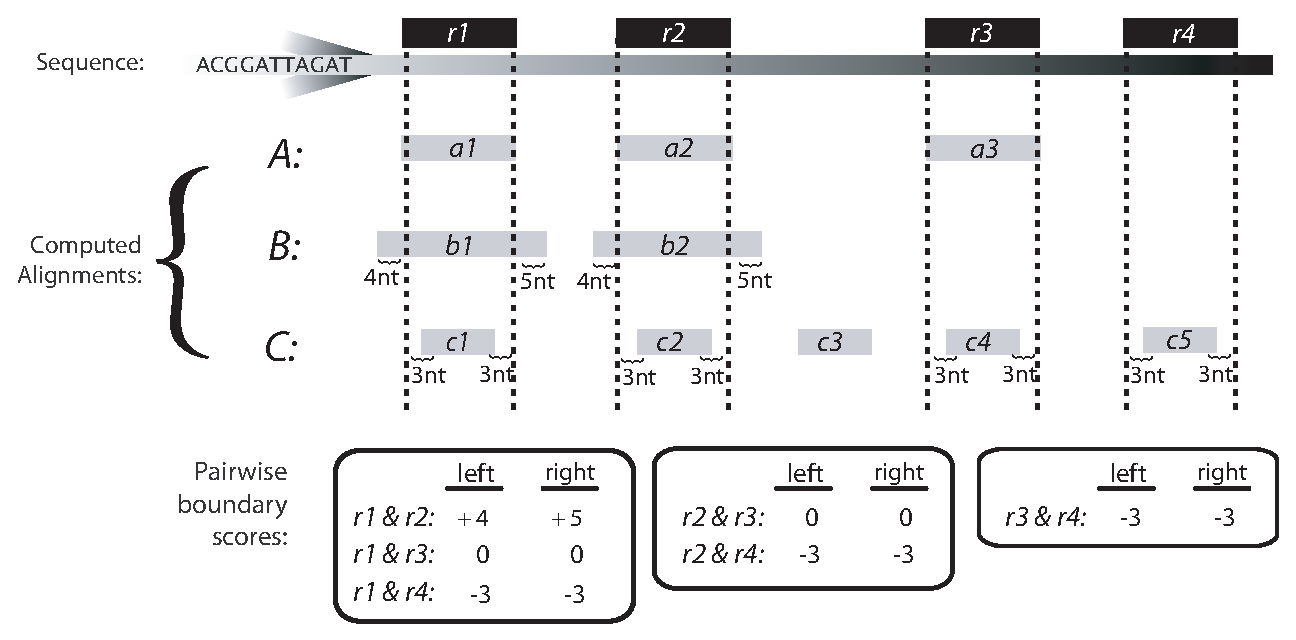
\epsfig{file=./fig/boundary_scores.eps,width=6.5in}
\caption[Pairwise boundary accuracy metric]%
{\textbf{Pairwise boundary accuracy metric}. We define our boundary accuracy metric to be an all-pairs score by comparing the boundaries of all \emph{r} components of the inserted repeat \emph{R} to the boundaries predicted by the alignment program. For any pair of components, $\emph{r}_{i}$ and $\emph{r}_{j}$, we take the maximum boundary of any local multiple alignments output by the program. The figure shows a multiplicity five interspersed repeat \emph{R} and four local multiple alignments, \emph{A, B, C, D}.  Boundary predictions can be classified as (1) correct, (2) overprediction, and (3) underprediction, with each discussed in turn: (1) \emph{Correct prediction}. Consider scoring components \emph{r1} and \emph{r3}.  Local multiple alignment \emph{A} overlaps both \emph{r1} and \emph{r3} and no other alignment overlaps both \emph{r1} and \emph{r3}.  The left and right boundaries of alignment \emph{A} match the boundaries of \emph{r1\&r3} exactly, thus we assign scores of 0 for \emph{r1\&r3}.  (2) \emph{Overprediction}. Consider scoring components \emph{r1} and \emph{r2}.  These components are overlapped by alignments \emph{A} and \emph{C}.  Alignment \emph{A} has perfect boundary predictions for \emph{r1\&r2}, while alignment \emph{C} extends beyond the true boundaries of components \emph{r1} and \emph{r2} by 4 nucleotides on the left and 5 nucleotides on the right.  Our scoring metric always uses the maximum predicted boundaries for a pair of components, thus the boundary predictions from \emph{C} are reported for \emph{r1\&r2}. (3) \emph{Underprediction.}  Consider scoring components \emph{r3} and \emph{r5}.  Alignment \emph{B} hits both \emph{r3} and \emph{r5}, but stops short of the right-side boundary by 8nt in \emph{r3} and 4nt in \emph{r5}.  We average the error and record -6 for the right-side of \emph{r3\&r5}.
Finally, component pairs that are not contained by any computed alignments are not scored, as indicated by \emph{n/a}.}
\label{fig-overunder}
\end{figure*}
\section{Results}
We have previously demonstrated the sensitivity of our chaining method
in finding Alu repeats in the human
genome~\cite{ref-procrast}. To highlight the benefits of our proposed
heuristic for gapped extension, we compare the performance of the implementation of our method ( ~\texttt{Repeatoire}) to the Eulerian path method for local multiple alignment
as implemented by \texttt{EulerAlign}~\cite{ref-related1}. The Eulerian
path method uses a \textit{de Bruijn} graph for filtration, and goes
beyond filtration to compute gapped alignments using banded dynamic
programming.  To the best of our knowledge, \texttt{Repeatoire} and
\texttt{EulerAlign} represent the only two automated methods to directly
construct local multiple alignments of \emph{generic} repeat families from genomic DNA.


\subsection*{Simulating interspersed repeats}
We evaluate accuracy of each method when aligning simulated repeat
families that have been inserted into the complete genome of
\emph{Mycoplasma genitalium}. The \emph{M. genitalium} genome has been recognized
as complex and repeat-rich, presenting a biologically
relevant and challenging example to evaluate alignment
methods~\cite{ref-mycoplasma}. We simulated repeat families of 8
different multiplicities ranging between 2 and 256 ($x$-axis in
Figure~\ref{fig-results}).  Each repeat copy has an average length
based on its family's multiplicity
($length=\frac{7680}{multiplicity}$), thus high copy-number repeats
are short.  The length of each repeat for each multiplicity was chosen
to reflect common repeat families found in genomes. Evolution of repeat families was simulated as a marked
Poisson process on a star tree
topology.  The branch lengths were varied between 0 and 24 ($y$-axis
in Figure~\ref{fig-results}), with the nucleotide substitution rate
fixed at 0.09 per unit time, and the indel rate fixed at 0.01 per
unit time.  Rate heterogeneity among sites was modeled with a gamma
distribution ($\theta = 1.0, k = 0.5$).  Indel size was
Poisson distributed with intensity 3, and insertions and deletions
were taken to be equally likely.  Each family's ancestral
sequence was randomly generated using nucleotide frequencies equal to
the composition of \emph{Mycoplasma genitalium}
($A=0.34,T=0.34,G=0.16,C=0.16$). Insertion sites for repeat copies
were chosen uniformly at random in the 580kb \textit{M. genitalium} genome,
allowing tandem repeats but prohibiting mosaic repeats. It is important to note that some or all copies of the simulated repeat families
could possibly be inserted inside of larger existing repeats in the  \textit{M. genitalium} genome, which would
likely result in each repeat detection program overextending the boundaries and scored as such. However, we make the assumption
that such cases would equally affect the boundary accuracy of each program and thus take no additional measure to account for inserting
artificial repeats into the complex genomic landscape of \textit{M. genitalium}.
\begin{figure*}[t!]
\centering
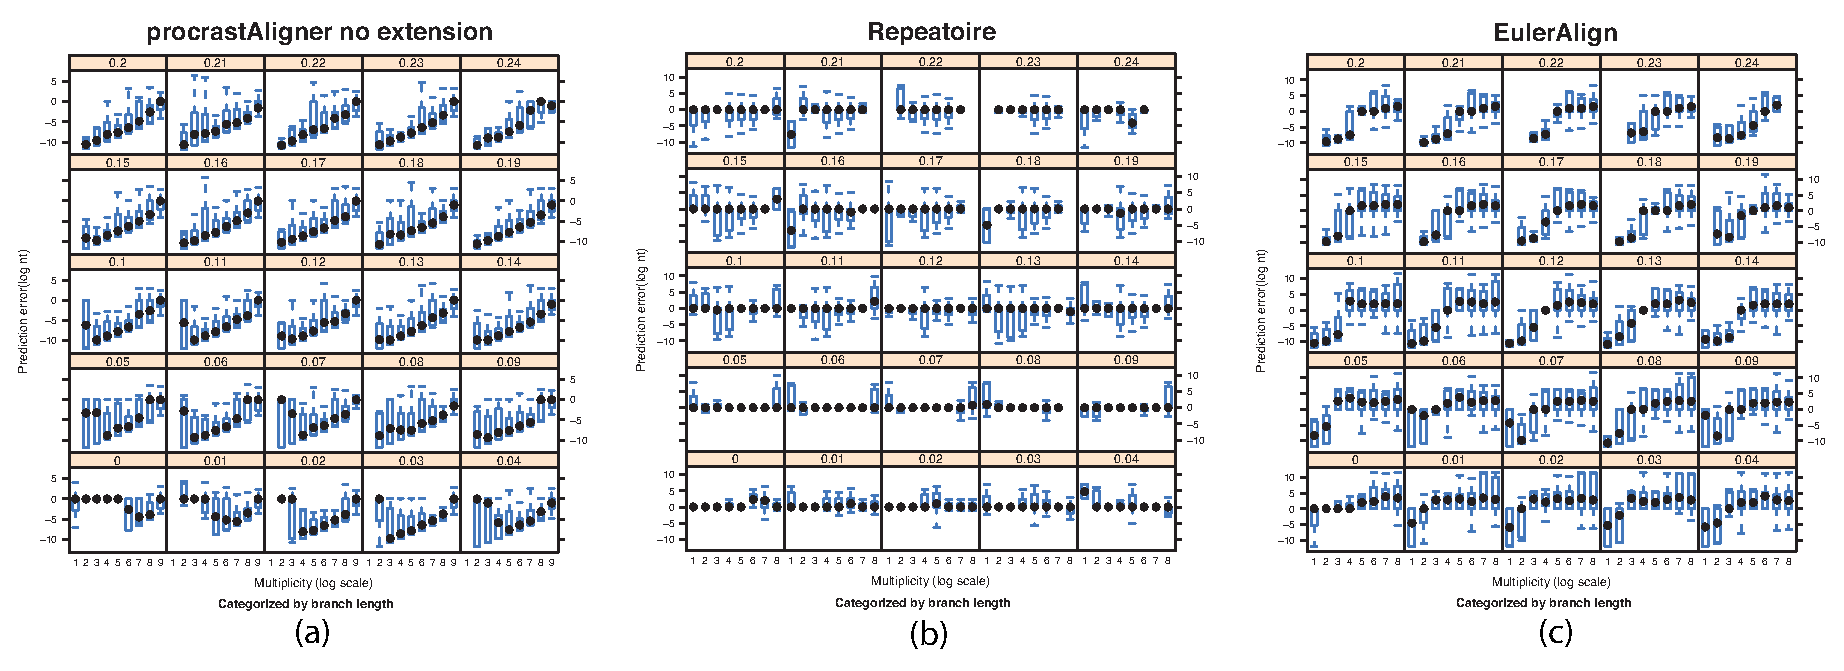
\epsfig{file=./fig/boundaryresults.eps,width=6.5in}
\label{fig:subfig1}
\caption[Boundary prediction performance]%
{\textbf{Boundary prediction performance}. All-pairs boundary prediction accuracy of \texttt{Repeatoire} and \texttt{EulerAlign} were measured for 200 combinations of branch length and multiplicity.  To give a better idea of the benefits of gapped extension we have included a comparison to a previous version of our algorithm which performed chaining but not gapped extension (indicated by procrastAligner no extension). Accuracy on each combination is presented as a box-and-whiskers plot using the scoring metric detailed in Section~\ref{sec:metrics}.  Branch lengths range from 0 to 0.24 and increase by intervals of 0.01.  The $x$-axis label represents the multiplicity of the interspersed repeat in log$_2$-scale. i.e. axis label 8 indicates $2^{8}$ = multiplicity 256. The $y$-axis label is the prediction error in log$_2$-scale nucleotides. Values at 0 represent correctly identified repeat boundaries, values greater than 0 represent overpredictions, and values less than 0 represent underpredictions (see Figure~\ref{fig-overunder}). In general, \texttt{Repeatoire} identifies the true interspersed repeat boundaries more accurately than \texttt{EulerAlign}.}
\label{fig-boundary}
\end{figure*}
\subsection*{Alignment accuracy metrics}
\label{sec:metrics}
We used each program to find local multiple alignments in each of the
200 modified \emph{M. genitalium} genomes and recorded alignment
accuracy as follows. We calculated sum-of-pairs nucleotide sensitivity
as $\frac{\mathrm{TP}}{\mathrm{TP} + \mathrm{FN}}$, where
$\mathrm{TP}$ is the number of aligned nucleotide pairs in the
program's output which are also aligned in the simulated repeat
family.  $\mathrm{FN}$ is the number of aligned nucleotide pairs in
the simulated repeat family which are missing from the program's
output.  This sensitivity measure is identical to the Sum-of-Pairs
accuracy defined by BaliBASE~\cite{ref-balibase}.  We calculate the
positive predictive value (PPV) as $\frac{\mathrm{TP}}{\mathrm{TP} +
\mathrm{FP}}$, where $\mathrm{TP}$ is defined as above, and
$\mathrm{FP}$ is the total number of nucleotide pairs from the
program's output where one of the nucleotides are part of the
simulated repeat family and the other nucleotide was incorrectly
aligned. We also quantify the ability of each aligner to accurately predict the
boundaries of the interspersed repeats.  For a given pair of repeat components, we calculate accuracy by recording the number of nucleotides between the true boundary and the predicted boundary
on both the right and left sides of the repeat.  Thus, over-extension gets a positive score, while underextension
yields a negative score and perfect boundaries receive a 0 score. See Figure~\ref{fig-overunder} for
further details on boundary under/overpredictions.


\subsection*{Accuracy when aligning interspersed repeats}
We applied \texttt{Repeatoire} and \texttt{EulerAlign} to the
hybrid simulated/real dataset.  We ran \texttt{Repeatoire}
with command-line parameters \texttt{--z=15 --w=20}, and
\texttt{EulerAlign} with \texttt{-k 15 -l -i 1000 -v} based on suggestions
from the program's user guide and manual experimentation.
Simulations for each of the 200 combinations of branch length and
multiplicity were replicated three times and alignments generated in
parallel on a 156-node computer cluster.  Also, we adapted the default \texttt{Repeatoire} HMM emission probabilities based on HOXD70 to 95\% sequence identity (\texttt{--percentid=0.95}), since the default 65-70\% identity would be too low for the majority of mutation rates.  Results of the experiments
are reported in Figure~\ref{fig-results} and
Figure~\ref{fig-boundary}. Figure~\ref{fig-results} illustrates the
sensitivity and PPV of
\texttt{Repeatoire} and
\texttt{EulerAlign} on datasets ranging from 0 substitutions and
indels per site to 2.16 substitutions and 0.24 indels per site (branch length 24).  As
mutation rates and repeat multiplicity increase the alignment accuracy
decreases for both methods, with accuracy of \texttt{EulerAlign}
decreasing faster than \texttt{Repeatoire}.  However, \texttt{EulerAlign}
often fails to fully align low multiplicity repeats, even when mutation rates are low.
Manual experimentation with \texttt{EulerAlign} parameters, such as: -v (tolerance for mismatches), -k (seed $k$-mer size) from 11 to 15, and -i (number of iterations) from 1000 up to 10,000, failed to improve its performance on low-multiplicity repeats.
We conjecture that \texttt{Repeatoire}'s overall improved accuracy largely derives
from its use of spaced seed patterns~\cite{ref-procrast} and tolerance
of gaps. With the \texttt{-v} option enabled, the Eulerian path method allows up to 10\% mismatches for matching $k$-mers to seed gapped alignment extensions. While this certainly improves the sensitivity at lower mutation rates, the experimental results presented Figure~\ref{fig-results} show that it is inadequate for higher mutation rates. In addition to sensitivity and PPV benchmarks, we also assess how well
each aligner recovers the true boundaries of interspersed
repeats.  Figure~\ref{fig-boundary} illustrates the ability of each
program to accurately localize the known boundaries of the simulated interspersed
repeats. From the figure, we first see the benefits of gapped extension when comparing our previous work
that did not perform gapped extension. For low multiplicities (2 to 4) and low mutation rates (0 to 0.05), procrastAligner performs as well
as the gapped extension algorithm implemented in Repeatoire, which can be attributed to the sensitivity offered by using palindromic seeds. Worth noting is that even when there is no mutations, procrastAligner can result in underextended boundaries. This can be explained due the the default seed size is small (15 nt) and can result in spurious matches or matching existing repeats in the reference genome, which will lead to underextended boundaries in spite of low mutation rates. However, once the repeat multiplicity or mutation rates increase, there is severe deterioration in the boundary predication accuracy, resulting in significant underprediction of the true boundaries.

When comparing both gapped extension algorithms, \texttt{EulerAlign} and \texttt{Repeatoire}, we found that \texttt{Repeatoire} more accurately predict
the repeat boundaries for all studied combinations of branch length (repeat degeneracy)
and multiplicity (repeat copy number).  Moreover, the standard error in \texttt{Repeatoire}'s
boundary predictions is typically very low, often within a few nucleotides of the true boundaries.  \texttt{EulerAlign}, on the other hand,
exhibits more erratic behavior.  For low multiplicity repeats it has a strong tendency to
underpredict the repeat boundaries.  At high multiplicities ($\geq32$) \texttt{EulerAlign} tends to
slightly overpredict the boundaries, by including flanking unrelated sequence in the alignment of
the interspersed repeat.  And as expected, when using the default \texttt{Repeatoire} HMM emission probabilities resulted in no underpredictions, although the overpredictions were more abundant (data not shown).

%We would like to extend this analysis to more closely compare the performance of boundary prediction accuracy of merging pairwise alignments into repeat families to that of directly constructing multiple alignments.
%\subsection{Runtime comparison}

Finally, a direct comparison of run time is difficult, due to the differing natures of the local multiple alignment programs.  \texttt{EulerAlign} runtime depends on the iterations parameter, which controls the total number of local multiple alignments reported, whereas \texttt{Repeatoire} reports \textit{all} local multiple alignments in a single run.  Despite this, we report the average per-experiment CPU time for each program on the test dataset. \texttt{Repeatoire} required on average 55 seconds per experiment, with the longest taking just over two minutes. \texttt{EulerAlign} required 1 hour total compute time per experiment on average, which equates to about 4 seconds per iteration.  Both programs exhibited similar memory usage, \texttt{Repeatoire} requiring on average 50 MB per experiment and \texttt{EulerAlign} requiring on average 70 MB per experiment.

\section{Estimating significance of local multiple alignments}
Increased seed matching sensitivity creates additional
false positive seed hits, so a statistical test for rejecting
insignificant local alignments is essential.  BLAST statistics have proven
invaluable for assessing the significance of pairwise local alignments, for amino acid and nucleotide sequences.
Fast methods to approximate the significance of pairwise
repeats have been implemented~\cite{repseek} and potentially can be
extended to multiple alignments~\cite{ref-related1, Prakash2005}.  We
now describe the method we use for estimating significance of local
multiple alignments.

For the present work, we are not concerned with random similarity between two or more sequences, but rather, random similarity arising within a single sequence.  We would like to compute the likelihood that a given repeat would appear by chance in order to decide whether the repeat reflects true sequence homology or random similarity.  Much effort has been expended to derive the probability of finding a segment of score $S$ between two sequences (see~\cite{Ewens2001} and references therein) or shared by $k$ sequences~\cite{ref-related1}. These statistics~\cite{Karlin1990} show that, $N$, the number of high scoring similarity segments between two sequences of size $m$ and $n$ with a score $S \geq x$ converges to:

\begin{equation}
    E[ N_{(S\geq x)} ] = Kmn p^x
    \label{E_mn}
\end{equation}

$K$ is a scale parameter that depends on the scoring system and $p$ (also often seen as $p=e^{-\lambda}$) can be understood as the per site probability of finding a segment of score 1. Using a Poisson approximation, the probability that the largest score is greater than or equal to $x$ is given by:

\begin{equation}
    P( S_1 \geq x) = 1 - exp( -E[ N_{(S\geq x)} ] )
    \label{P_s1}
\end{equation}

For gap-free alignments, both parameters $K$ and $p$ can be computed numerically~\cite{Karlin1990} whereas their estimation relies on simulations when gaps are allowed  ~\cite{Waterman1994, Altschul2001}.

The above statistics to compute expectation of matching across two sequences can be easily extended to 2-copy repeats within the same strand of a sequence of size $n$, by substituting $mn$ by ${{n}\choose{2}}$ in the above equations. Taking both strands of DNA into account, we have to count successively cases where 0, 1 or 2 copies are on the forward strand; copies on the same strand can be swapped without changing the repeat structure. Therefore, the expected number of 2-copy repeats on both strands with a score greater or equal than $x$ is:

\begin{eqnarray}
   E[ N_{(r=2, S\geq x)} ]  & = & K \times  \Big( n (n-1) \frac 12 (\frac 1 2 + 1 + \frac 1 2) \Big) \times  p^x \nonumber \\
                                         & = & K  n (n-1)   p^x
   \label{E_r2}
\end{eqnarray}

This assumes that repeats cannot begin at the same positions neither in the same or in the opposite strand ($i.e.$ $n(n-1)$). Furthermore, because of the strand symmetry, when one counts repeats where both copies are in the forward strand, one also includes repeats with both copies in the reverse strand. Therefore, the searching space is in the order of $O(n^2)$ along with a factor $\frac 12 (\frac 1 2 + 1 + \frac 1 2)$ that corrects for the multiple counts of the same repeats. More generally, the expected number of repeats of multiplicity $r$ on both strands that have a score greater than or equal to $x$ is given by:

\begin{equation}
    E[ N_{(r, S\geq x)} ]   =  K \times  \Big( \frac{n!}{(n-r)! }  \frac 12 \sum_{k=0}^{r}{\frac{1}{k! (r-k)!}} \Big) \times  p^{(r-1)x}
    \label{E_repeat}
\end{equation}

In the above equation, the two unknown parameters $K$ and $p$ can be estimated on 2-copy repeats using random sequences of the same size and identical composition.  This can be done by using either the direct method~\cite{Olsen1999} with a $log(-log(1-P))$ transformation of the Equation \ref{P_s1}, or by using the declumping method ~\cite{Waterman1994}, or by the island method~\cite{Olsen1999} using a $log(E)$ of Equation \ref{E_r2}. Once $K$ and $p$ are estimated, Equation \ref{P_s1} along with Equation \ref{E_repeat} can be used to asses the probability of any observed repeat of a given score and a given multiplicity. An adequate score to be used is the average pairwise alignment score of repeat components.

%Importantly, these equations show a perfect fit with repeats from random genomes (data not shown).

Although our significance measure for local multiple alignments is only an approximation, its introduction will allow
for increased sensitivity (i.e. smaller seed size, seed families) while maintaining specificity. The statistical
test helps to filter out spurious alignments, although it doesn't resolve redundant alignments. To address redundant alignments, we follow
the approached proposed in~\cite{ref-related1} by grouping all alignments which share at least one aligned column. Then, we can select the reference alignment
as the alignment in the group with the highest Sum-of-Pairs (SP) score, breaking ties either by multiplicity or repeat length. The selection of a reference alignment from each redundant group can be defined by the user via a command-line parameter, allowing for the reference alignment to be tailored towards specific repeat analysis tasks.



\section{Conclusion}
We have presented a sensitive and efficient gapped-extension heuristic for local
multiple alignment. We have extended our results implemented in previous work (\texttt{procrastAligner}) by
converting chains of ungapped multi-matches into gapped local multiple
alignments through steps (C) through (F) of the presented heuristic. We have also added a method to remove spurious local multiple alignments by introducing a statistical estimation of significance
performed directly on the input sequence. We have implemented our method in the \texttt{Repeatoire} software. Experimental results demonstrate that the
described method offers a level of alignment accuracy exceeding
that of a related method. 

Accurately predicting homology boundaries has important implications; for example, tools to build repeat family databases can directly use the alignments without the manual curation required in current approaches and also is likely to aid in the evolutionary analysis of repeat proliferation.  We also would like to emphasize the importance of correctly selecting an appropriate substitution matrix for the expected amount of divergency among the repeats. The default substitution matrix our program uses is the HOXD70 matrix, which is optimized for 70\% sequence identity. Thus, using the default substitution matrix when performing repeat detection on less diverged families can result in overextended repeat boundaries, or vice versa.

An improvement of our gap open and gap extension emission parameters in the Homologous state would be to better represent the indel spectra in coding/non-coding regions by considering both. Further improvement of the alignment methodology will likely require increasingly sensitive methods for
seed matching. One possible avenue to increase seed matching sensitivity and reduce boundary underpredictions would be merging overlapping seed matches into a
shorter, higher-multiplicity match.  A second avenue would be to use palindromic seed families instead of using a single seed pattern~\cite{ref-pattern}.

\subsection*{Implementation}
We have implemented our method in a program, \texttt{Repeatoire},
available for Linux, Windows, and Mac OS X. Our open-source
implementation is available as C++ source code licensed under the GPL , and can be downloaded from: \\
\url{http://wwwabi.snv.jussieu.fr/public/Repeatoire}.

\section{ Acknowledgment }
The authors would like to thank Y Zhang for providing the
\texttt{EulerAlign} program for evaluation. We would also like to thank
W Miller for providing the HOXD70 substitution matrix data. Others to thank... Accuracy
evaluations utilized a compute resource grant from the Australian
Partnership for Advanced Computing.  AED was supported by NSF grant
DBI-0630765. TJT was supported in part by Spanish Ministry MECD Grant
TIN2004-03382.

% trigger a \newpage just before the given reference
% number - used to balance the columns on the last page
% adjust value as needed - may need to be readjusted if
% the document is modified later
%\IEEEtriggeratref{8}
% The "triggered" command can be changed if desired:
%\IEEEtriggercmd{\enlargethispage{-5in}}

% references section
% NOTE: BibTeX documentation can be easily obtained at:
% http://www.ctan.org/tex-archive/biblio/bibtex/contrib/doc/

% can use a bibliography generated by BibTeX as a .bbl file
% standard IEEE bibliography style from:
% http://www.ctan.org/tex-archive/macros/latex/contrib/supported/IEEEtran/
%\bibliographystyle{IEEEtran.bst}
% argument is your BibTeX string definitions and bibliography database(s)
%\bibliography{IEEEabrv,../bib/paper}
%
% <OR> manually copy in the resultant .bbl file
% set second argument of \begin to the number of references
% (used to reserve space for the reference number labels box)

\bibliographystyle{IEEEtran}
\bibliography{procrastination}
\appendix[Supplemental Material]
\thispagestyle{empty}
\subsection*{Calculating emission probabilities from the HOXD70 substitution matrix}
We will now outline how we have dervied the HMM emission probabilities using the HOXD70 substitution matrix. First, given that the training
data has $47.5\%$~$G+C$ content and considering reversibility of the substitution process, we can compute emission probabilities for the Unrelated state
of our HMM:
\begin{multline}\\
U_{AA}=U_{AT}=U_{TA}=U_{TT}=(\frac{f_{AT}}{2})(\frac{f_{AT}}{2})
= 0.06890625 \\
U_{CC}=U_{CG}=U_{GC}=U_{GG}=(\frac{f_{GC}}{2})(\frac{f_{GC}}{2}) =
0.05640625 \\
U_{AC}=U_{AG}=U_{TC}=U_{TG}=(\frac{f_{AT}}{2})(\frac{f_{GC}}{2}) =
0.06234375 \\
U_{CA}=U_{CT}=U_{GA}=U_{GT}=(\frac{f_{GC}}{2})(\frac{f_{AT}}{2}) =
0.06234375 \\
\label{eq-ff}
\end{multline}
Where $f_{GC}=0.475$ and $f_{AT}=0.525$ are background frequencies of
G/C and A/T, respectively and the notation $U_{XY}$ indicates the probability of observing nucleotide X aligned to
nucleotide Y in Unrelated sequence.    Note, each $f_{XY}$ is divided by 2 to yield the frequency of a single nucleotide from dinucleotide background frequencies.

By using Equation~\ref{eq-hoxd} (from Section~\ref{section-main}), we can derive emission probabilities for
the Homologous state as follows:
\begin{equation}
\log_{2}\bigg(\frac{H_{AA}}{U_{AA}}\bigg) = \frac{91}{\psi},
\end{equation}
where $\frac{1}{\psi}$ is the unknown scaling factor used to normalize $H_{CC}$ to 100. The full list of equations follows:
\begin{multline}\\
\log_{2}\bigg(\frac{H_{AC}}{U_{AC}}\bigg) = \frac{-114}{\psi}\\
\log_{2}\bigg(\frac{H_{AG}}{U_{AC}}\bigg) = \frac{-31}{\psi}\\
\log_{2}\bigg(\frac{H_{AT}}{U_{AC}}\bigg) = \frac{-123}{\psi}\\
\log_{2}\bigg(\frac{H_{CG}}{U_{CC}}\bigg) = \frac{-125}{\psi}\\
\log_{2}\bigg(\frac{H_{AA}}{U_{AA}}\bigg) = \frac{91}{\psi}\\
\log_{2}\bigg(\frac{H_{CC}}{U_{CC}}\bigg) = \frac{100}{\psi}\\
\end{multline}

The system of six equations has seven free variables.  Moreover, the $H_{xy}$ must sum to 1 to make a probability distribution:
\begin{equation}
2H_{AA} + 4H_{AC} + 4H_{AG} + 2H_{AT} + 2H_{CC} + 2H_{CG} = 1
\end{equation}
%$0.03072937146$
%$32.54215601$
We can solve the above six equations for $H_{xy}$ and substitute the
resulting expressions in to the normalizing equation to solve for
$\psi$. For the HOXD70 matrix the scaling factor is $\psi=66.667$. Given
$\psi$, we can calculate values for all $H_{xy}$.

\subsection*{Adapting HMM parameters to organisms with different G+C content}

Emission
probabilities in the Unrelated state can be directly adapted to the
background nucleotide distribution ($f_{GC}, f_{AT}$) using Equation~\ref{eq-ff}. To adapt emission probabilities in the homologous state, we consider the
probability of nucleotide substitution under the standard assumption
that sequences evolve according to a continuous-time reversible Markov process.
Thus, the probability of nucleotide $X$ mutating to nucleotide $Y$ over time $t$
can be written as:
\begin{equation}
H_{XY}=\pi_X \exp^{Q(X,Y)t}
\end{equation}
, where $\pi_X$ represents the background
frequency of nucleotide $X$ and $Q(X,Y)$ is the instantaneous substitution rate for $X$
mutating to $Y$. Important to note is that we make the assumption that the probability of
either nucleotide at the root node is equal to their background
frequencies in the sequence. Also, as do other existing methods that correct for composition bias using an adapted substitution matrix~\cite{repseek}, we explicitly assume $t$ to be 1.  Because the background frequencies on which the substitution matrix was computed are
known (e.g. 47.5\%GC for HOXD70), we can replace the $\pi_X$ from the HOXD70 matrix
with the $\pi'_X$ from the input genome as follows:

\begin{equation}
H'_{XY}=(\frac{\pi'_X}{\pi_X})  H_{XY}
\end{equation}
\thispagestyle{empty}
%DERIVATION HERE!!
Given that the substitution process is
strand-symmetric and reversible, we can thus compute adapted
emission probabilities for the Homologous state as follows:
\begin{multline}\\
H'_{AG}=H_{AG}\\
H'_{AC}=H_{AC}\\
H'_{AA}=(\frac{f'_{AT}}{f_{AT}})H_{AA}\\
H'_{AT}=(\frac{f'_{AT}}{f_{AT}})H_{AT}\\
H'_{CC}=(\frac{f'_{GC}}{f_{GC}})H_{CC}\\
H'_{CG}=(\frac{f'_{GC}}{f_{GC}})H_{CG}\\
\end{multline}
where $f'_{AT}$ and $f'_{GC}$ represent the input genome's AT and GC content,
$H_{XY}$ values are the original emission probabilities derived from the
substitution matrix, and $H'_{XY}$ are emission probabilities adapted to
the input genome's G+C content.


%\section{Configuring the transition probabilities of the HMM}



% You can push biographies down or up by placing
% a \vfill before or after them. The appropriate
% use of \vfill depends on what kind of text is
% on the last page and whether or not the columns
% are being equalized.

%\vfill

% Can be used to pull up biographies so that the bottom of the last one
% is flush with the other column.
%\enlargethispage{-5in}

% that's all folks
\end{document}
